\documentclass[a4paper, 12pt]{article}
\usepackage{CJKutf8}
\usepackage{graphicx}

\title{analyze 'timer.c' in pjsip}
\author{icefreedom}
\date{\today}


\begin{document}
\maketitle

\begin{CJK}{UTF8}{gkai}

\section{Introduction}
在PJSIP中,timer的作用是定时发送sip消息, 它的原理有点类似twisted(python写的异步事件处理框架)中的reactor机制, 但timer是在单线程中处理事件, 在timer.c的文档中。
本文将分析timer的数据结构,原理,以及同reactor机制的比较。

\section{Data structure}
在timer.c的文档中对其数据结构的说明是a heap is a "partially ordered, almost complete" binary tree. 本质上,用的是二叉树, 它有两点特性: 
partially ordered, 部分有序,指的是父结点的time value 小于等于子结点, 但子结点是无序的; almost complete, 几乎是完全二叉树,指的是最后的结点
可能只有一个子结点。这两点在下面的分析中会看到。

\begin{enumerate}
\item
timer entry 被保存在一个数组中,称作heap, 是一个二叉树, timer entry中有一个timer id,
它是用来对timer entry索引的, 即用timer id可以快速找到timer entry,  如下图: \\
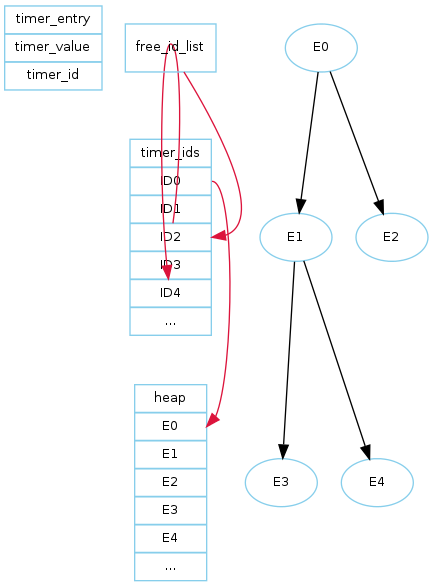
\includegraphics{timerdatastructure.png}

\item
增加timer entry的操作流程:1.分配timer id, 2. 将它加入heap最后的新结点,3. 向上移(reheap\_up)该结点到合适的位置,即保证父结点的timer value小于等于子结点的,
4. 记录其slot到timerIds中, 如下图:\\
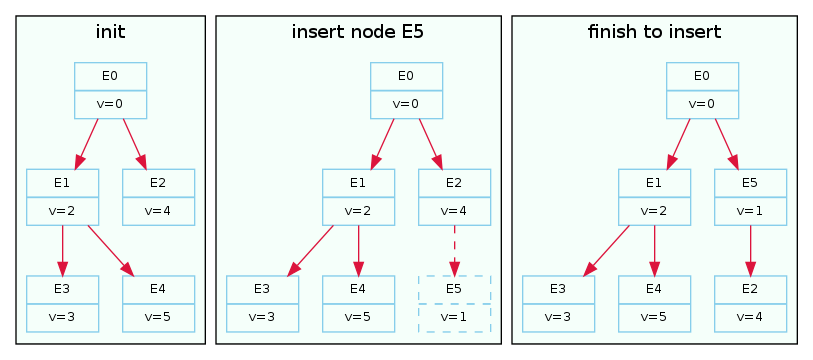
\includegraphics[width=\textwidth]{timerinsertnode.png}

\item
删除timer entry的操作流程: 1. 回收timer id 2.将heap最末的结点放到该结点位置,  3. 向上或向下移(reheap\_down)此结点到合适的位置, 如下图:\\
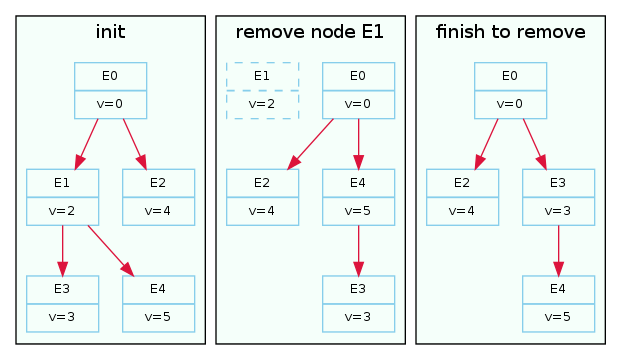
\includegraphics[width=\textwidth]{timerremovenode.png}

\end{enumerate}

\section{Interface}
timer.c中提供的接口主要有两个: poll和schedule,  
poll的作用是从heap中取出所有已经到时的timer entry, 这个在pjsua 的worker thread中循环调用
schedule就是插入一个timer entry, 并设定时间。

\section{Diff}



\end{CJK}

\end{document}